% !TeX program = xelatex
\documentclass[UTF8,11pt,a4paper,fontset=none]{ctexart}

% ---------- 页面与字体 ----------
\usepackage{geometry}
\geometry{left=2.4cm,right=2.4cm,top=2.6cm,bottom=2.5cm}
\setCJKmainfont[Path=fonts/,
  BoldFont=FandolSong-Bold.otf,
  ItalicFont=FZKai.ttf,
  BoldItalicFont=FandolSong-Bold.otf
]{FZShuSong.ttf}
\setCJKsansfont[Path=fonts/]{FZHei.ttf}
\setCJKmonofont[Path=fonts/,Scale=0.94]{FZShuSong.ttf}
\setCJKfamilyfont{kaishu}[Path=fonts/,BoldFont=FandolSong-Bold.otf]{FZKai.ttf}
\ctexset{
  section = {format = \Large\sffamily\raggedright},
  subsection = {format = \large\sffamily\raggedright},
  subsubsection = {format = \normalsize\sffamily\raggedright}
}
\setmainfont{Times New Roman}
\setsansfont{Noto Sans CJK SC}
\setmonofont{DejaVu Sans Mono}
\linespread{1.28}
\setlength{\parindent}{2em}
\setlength{\parskip}{0.25em}
\setlength{\headheight}{13pt}

% ---------- 数学、图表、代码 ----------
\usepackage{amsmath,amssymb,bm}
\usepackage{graphicx}
\usepackage{booktabs}
\usepackage{longtable}
\usepackage{array}
\usepackage{multirow}
\usepackage{makecell}
\usepackage{float}
\usepackage{caption}
\usepackage{subcaption}
\usepackage{xcolor}
\usepackage{listings}
\usepackage{fancyhdr}
\usepackage{enumitem}
\usepackage{needspace}
\usepackage{titlesec}
\usepackage[hidelinks]{hyperref}
\usepackage{url}

\definecolor{deepgreen}{RGB}{18,59,50}
\definecolor{accent}{RGB}{47,125,104}
\definecolor{codebg}{RGB}{247,249,248}
\definecolor{codegray}{RGB}{110,110,110}
\definecolor{codeblue}{RGB}{30,70,140}
\definecolor{codegreen}{RGB}{30,110,80}
\definecolor{rulegray}{RGB}{180,190,186}

\captionsetup{font={small,sf},labelfont=sf,labelsep=quad}
\captionsetup[table]{skip=4pt}
\setlist[itemize]{leftmargin=2em,itemsep=0.2em,topsep=0.2em}
\setlist[enumerate]{leftmargin=2em,itemsep=0pt,parsep=0pt,topsep=0pt,partopsep=0pt,before=\vspace{-\parskip},after=\vspace{-\parskip}}
\AtBeginDocument{%
  \setlength{\abovedisplayskip}{2pt plus 0pt minus 0pt}%
  \setlength{\belowdisplayskip}{2pt plus 0pt minus 0pt}%
  \setlength{\abovedisplayshortskip}{0pt plus 0pt minus 0pt}%
  \setlength{\belowdisplayshortskip}{0pt plus 0pt minus 0pt}%
}

\lstdefinelanguage{JavaScript}{
  keywords={const,let,var,function,return,await,async,new,true,false,null,undefined,if,else,for,while,throw,try,catch},
  sensitive=true,
  comment=[l]{//},
  morecomment=[s]{/*}{*/},
  morestring=[b]',
  morestring=[b]",
  morestring=[b]`
}
\lstdefinestyle{papercode}{
  basicstyle=\ttfamily\small,
  keywordstyle=\color{codeblue}\bfseries,
  stringstyle=\color{codegreen},
  commentstyle=\color{codegray}\upshape,
  breaklines=true,
  breakatwhitespace=false,
  columns=fullflexible,
  keepspaces=true,
  frame=single,
  rulecolor=\color{rulegray},
  backgroundcolor=\color{codebg},
  showstringspaces=false,
  tabsize=2,
  numbers=left,
  numberstyle=\tiny\color{codegray},
  numbersep=6pt,
  xleftmargin=2.2em,
  framexleftmargin=1.6em,
  captionpos=b,
  breakindent=2em,
  aboveskip=0.8em,
  belowskip=0.6em
}
\lstset{style=papercode}
\renewcommand{\lstlistingname}{代码}

% ---------- 页眉页脚 ----------
\pagestyle{fancy}
\fancyhf{}
\fancyhead[L]{\small 超级马里奥 · AI Water}
\fancyhead[R]{\small CIE RISC-V 大赛}
\fancyfoot[C]{\small \thepage}
\renewcommand{\headrulewidth}{0.4pt}
\fancypagestyle{plain}{
  \fancyhf{}
  \fancyfoot[C]{\small \thepage}
  \renewcommand{\headrulewidth}{0pt}
}

% ---------- 标题信息 ----------
\title{\bfseries 面向绿色水务的 RISC-V 边缘多模态检漏终端\\[0.4em]
\large 基于进迭时空 K1 的声学感知、语音交互与碳效评估}
\author{超级马里奥\\
\small 代码仓库：\url{https://github.com/Lvshujun0918/AI_Water}}
\date{2026 年 11 月}

\begin{document}
\maketitle
\thispagestyle{plain}

% ---------- 摘要 ----------
\begin{abstract}
{\CJKfamily{kaishu}
\noindent
城市供水管网漏损是一个被低估的“水—能—碳”问题：漏掉的水在到达用户之前，已经经历了取水、处理、加压输送，漏损因此同时意味着水资源浪费、电力消耗和碳排放。世界银行估计全球城市供水系统每年物理漏损约 320 亿立方米\cite{worldbank}；中国 2022 年城市公共供水漏损率为 12.89\%，2023 年降至 10\% 以内\cite{pingdingshan,gmw}。现有检漏主要依赖人工听音、相关仪和压力/流量分析，存在到达现场慢、依赖经验、难以规模化的问题。

本文以进迭时空 K1 为算力底座，设计并实现一台面向阀井、泵房和二次供水节点的边缘智能终端。系统以麦克风阵列采集管网声学信号，用 ResNetSE 声学事件识别模型在本地判断高风险、低风险和无风险；以语音识别把现场口令转为结构化意图；以本地小参数大模型解释风险、生成工单并回答运维问题；所有结果写入本地碳账本，形成可审计的“漏点—水量—电耗—碳排”证据链。工程的核心是建立一套可复现的 RISC-V 深度学习运行时：以 Bianbu 为基座，锁定进迭时空 wheel 源中的 PyTorch 2.8.0、torchvision 0.23.0、torchaudio 2.8.0，移除 yeaudio、librosa、scipy、numba 在推理主路径上的脆弱依赖，用 torchaudio 与 soundfile 重写 \texttt{AudioSegment}，并通过 Docker 与 GitHub Actions 交付可复现镜像。

本文给出系统架构、声学模型与训练细节、快慢双路径交互、RISC-V 适配代码、性能优化方案、绿碳核算模型、部署与测试方法。设计目标是常见语音指令端到端时延不超过 1 s，声学识别准确率不低于 90\%，整机离线运行，典型功耗不超过 15 W。实证了国产优秀进迭时空RISC-V环境在智慧水务上的应用价值。

\vspace{0.8em}
\noindent\textbf{关键词：} RISC-V；K1；边缘人工智能；供水管网；声学检漏；多模态交互；绿碳
}
\end{abstract}

% =====================================================================
\section{引言}
\label{sec:intro}

供水管网是城市基础设施中最庞大、最隐蔽的资产之一。管道埋在地下，泄漏初期的地表迹象通常滞后，等到路面塌陷或居民水压下降时，损失已经扩大。世界银行的研究给出的全球物理漏损量约为每年 320 亿立方米，发展中国家每天约有 4500 万立方米的水在输配过程中损失\cite{worldbank}。这同时是一笔能源与碳的成本：水在被漏掉之前，已经经历了取水、混凝、沉淀、过滤、消毒和泵送。

中国的情况同样严峻。公开资料援引《2022 年城市建设统计年鉴》指出，2022 年全国城市供水 635.45 亿立方米，漏损水量 81.91 亿立方米，漏损率 12.89\%\cite{pingdingshan}；到 2023 年，城市公共供水管网漏损率下降到 10\% 以内\cite{gmw}。政策目标是到 2025 年全国城市公共供水管网漏损率力争控制在 9\% 以内\cite{mohurd}。从 12.89\% 降到 9\%，对应的是数十亿立方米的年节水量。

水与电在供水系统中高度耦合。国际能源署（IEA）估计，全球水部门（含取水、处理、输配和污水收集处理）消耗的电力约占全球总用电量的 4\%\cite{iea}。漏损的水是“已经花过电的水”：它被抽上来、处理过、加压送出去，最后从破口流走。减少漏损，等于同时减少取水、处理和泵送三个环节的能耗。本文把这一关系称为“水—能—碳耦合”，并把碳账本嵌入检漏终端，使每一个漏点都能折算成可复核的水量、电量和二氧化碳减排量。

现有检漏方法各有局限。人工听音依赖经验，夜间作业强度大；相关仪定位精度较高，但需要两处接触，操作复杂；压力/流量分区计量能发现区域异常，却难以定位微小泄漏；光纤、卫星和无人机覆盖范围大，但成本高，不适合室内泵房。云端音频分析模型能力强，但依赖网络、带宽和隐私合规，难以在阀井和地下泵房稳定工作。实际管网需要“分区计量发现异常、声学终端确认漏点、人工现场复核”的组合，本文聚焦其中最适合边缘部署的一环。

本文的贡献包括：

\begin{enumerate}
  \item 设计了一套面向供水管网的单板边缘终端架构，将声学感知、语音交互、本地语言模型和碳账本集成到 K1 平台，并给出快慢双路径的时延预算。
  \item 建立了团队自主维护的 RISC-V 深度学习运行时适配层：统一 wheel 源、固定版本、显式 ABI 路径、替换音频前端、移除 numba/librosa/scipy 推理依赖，并以容器和 CI 交付。
  \item 提出一种可审计的运行阶段碳核算方法，把漏点流量、提前发现时间、供水综合电耗和电网排放因子写入事件账本，并给出敏感性分析。
  \item 给出完整的实验设计与测试协议，包括准确率、时延、稳定性、功耗和异常恢复，明确区分已实现结果与待实测目标。
\end{enumerate}

本文其余部分安排如下：第\ref{sec:related}节讨论相关工作与问题定义；第\ref{sec:architecture}节给出系统架构；第\ref{sec:acoustic}节介绍声学感知方法；第\ref{sec:multimodal}节介绍多模态交互；第\ref{sec:riscv}节介绍 RISC-V 运行时适配；第\ref{sec:optimization}节讨论性能优化；第\ref{sec:carbon}节给出绿碳核算；第\ref{sec:evaluation}节给出部署与测试；第\ref{sec:discussion}节讨论局限；第\ref{sec:conclusion}节总结。

% =====================================================================
\section{相关工作与问题定义}
\label{sec:related}

\subsection{声学检漏}

声学检漏的基本原理是：高压水从破口喷出时形成湍流和空化，产生宽带噪声；声音沿管壁、土壤和空气传播，在阀门、消火栓、检查井等接触点可以被麦克风拾取。泄漏声的主要能量通常在几十赫兹到几千赫兹之间，具体频段受管材、管径、埋深、土壤湿度和水压影响。

传统方法依赖人工听音和相关分析。机器学习方法把声学检漏转化为分类或异常检测问题：提取 Mel 频谱、MFCC、Fbank 等特征，用卷积神经网络、ResNet、TDNN 或注意力模型分类。ResNetSE 在残差网络中加入 Squeeze-and-Excitation（SE）通道注意力\cite{se}，能够根据输入动态重标定通道，适合低信噪比、跨场景的声学任务。本文沿用这一思路，把重点放在边缘部署与运行时适配上。

\subsection{边缘多模态交互}

赛道要求 CV、ASR、LLM 中至少两种能力协同。本文选择“声学事件识别 + ASR + LLM”的路线，原因有三点。第一，声学感知是项目已有积累，能够直接复用到 K1；第二，ASR 可以在双手被占用的阀井场景提供自然交互；第三，本地 LLM 可以把风险证据转成工单和解释，降低对云端服务的依赖。CV 作为可选复核能力，只在声学高风险且摄像头可用时触发，避免持续视频推理抢占 CPU。

多模态融合的难点是确定“谁有最终决定权”。本文把 LLM 放在慢路径，把规则引擎放在快路径：ASR 识别指令后，规则引擎在毫秒级完成意图校验和动作白名单检查；LLM 只负责解释、工单和问答，不直接控制阀门或继电器。这样既保证交互时延，也避免大模型幻觉进入物理执行链路。

\subsection{问题定义}

给定一段 1--4 s 的管网音频 \(x\)，声学模型输出风险类别 \(y\in\{\text{高},\text{低},\text{无}\}\) 和置信度 \(p\)。给定一段语音 \(s\)，ASR 输出文本 \(t\)，意图解析输出指令 \(c\)。系统需要在本地完成：

\begin{equation}
  \hat{y}, \hat{p} = f_{\theta}(x), \qquad
  \hat{c} = g_{\phi}(s),
  \label{eq:problem}
\end{equation}

其中 \(\hat{y}\)、\(\hat{p}\) 和 \(\hat{c}\) 分别表示对应的预测值，\(\theta\) 和 \(\phi\) 分别表示声学模型和意图解析模型的参数；\(x\)、\(y\)、\(p\)、\(s\)、\(t\)、\(c\) 的含义已在上文给出。

并在满足时延、功耗、离线约束的前提下，输出告警、工单或碳账本条目。系统在 K1 的 2 TOPS 算力、8 GB 内存和低功耗约束下追求可用的端到端体验，模型精度服务于这一目标。

% =====================================================================
\section{系统架构}
\label{sec:architecture}

\subsection{硬件拓扑}

终端以 MUSE Pi Pro 为核心，按场景选配外设。K1 提供 8 个 X60 核、2 TOPS AI 算力、256-bit RVV 1.0 向量扩展、8 GB LPDDR4X 内存，以及 PCIe、USB 3.0、GMAC、MIPI DSI/CSI 和 40-pin GPIO\cite{spacemit}。表\ref{tab:hardware}给出典型配置。


终端可以做成桌面式（泵房）或防水盒式（阀井）。阀井版本需要额外考虑防潮、防凝露和麦克风防水膜；本文的软件方案不依赖具体外壳。

\subsection{软件分层}

系统自下而上分为五层，如图\ref{fig:arch}所示；图中箭头表示调用与数据依赖，不表示所有进程均常驻。

\begin{enumerate}
  \item \textbf{硬件层}：K1、麦克风、屏幕、摄像头、GPIO、通信模组。
  \item \textbf{运行时层}：Bianbu Linux、Python 3.12、Node.js 22、PyTorch 2.8.0、torchaudio 2.8.0、ONNX Runtime、llama.cpp。
  \item \textbf{智能层}：声学事件识别（AED）、语音识别（ASR）、本地大模型（LLM）、多模态融合与规则引擎。
  \item \textbf{服务层}：Express REST API、SQLite、任务队列、认证与审计。
  \item \textbf{交互层}：本地 Web 管理端、4.3 英寸触摸屏、语音、声光/继电器输出。
\end{enumerate}

\begin{table}[H]
\centering
\small
\caption{边缘终端硬件配置}
\label{tab:hardware}
\begin{tabular}{p{2.6cm}p{4.2cm}p{6.4cm}}
\toprule
部件 & 选型/接口 & 作用 \\
\midrule
主板 & MUSE Pi Pro，K1，8 GB & 本地推理、Web 服务、数据存储 \\
麦克风 & USB 阵列麦克风或模拟麦 + USB 声卡 & 采集 16 kHz 管网声音 \\
显示屏 & 4.3 英寸 MIPI DSI 触摸屏 & 现场告警、波形、工单确认 \\
摄像头 & OV5647，MIPI CSI（可选） & 高风险时拍照复核 \\
通信 & WiFi6 / 4G（miniPCIe） & 结构化结果回传 \\
存储 & eMMC + M.2 NVMe & 模型、音频证据、SQLite \\
执行 & 40-pin GPIO、继电器、蜂鸣器 & 声光告警与联动 \\
电源 & USB PD 3.0 & 单线供电 \\
\bottomrule
\end{tabular}
\end{table}

\begin{figure}[ht]
  \centering
  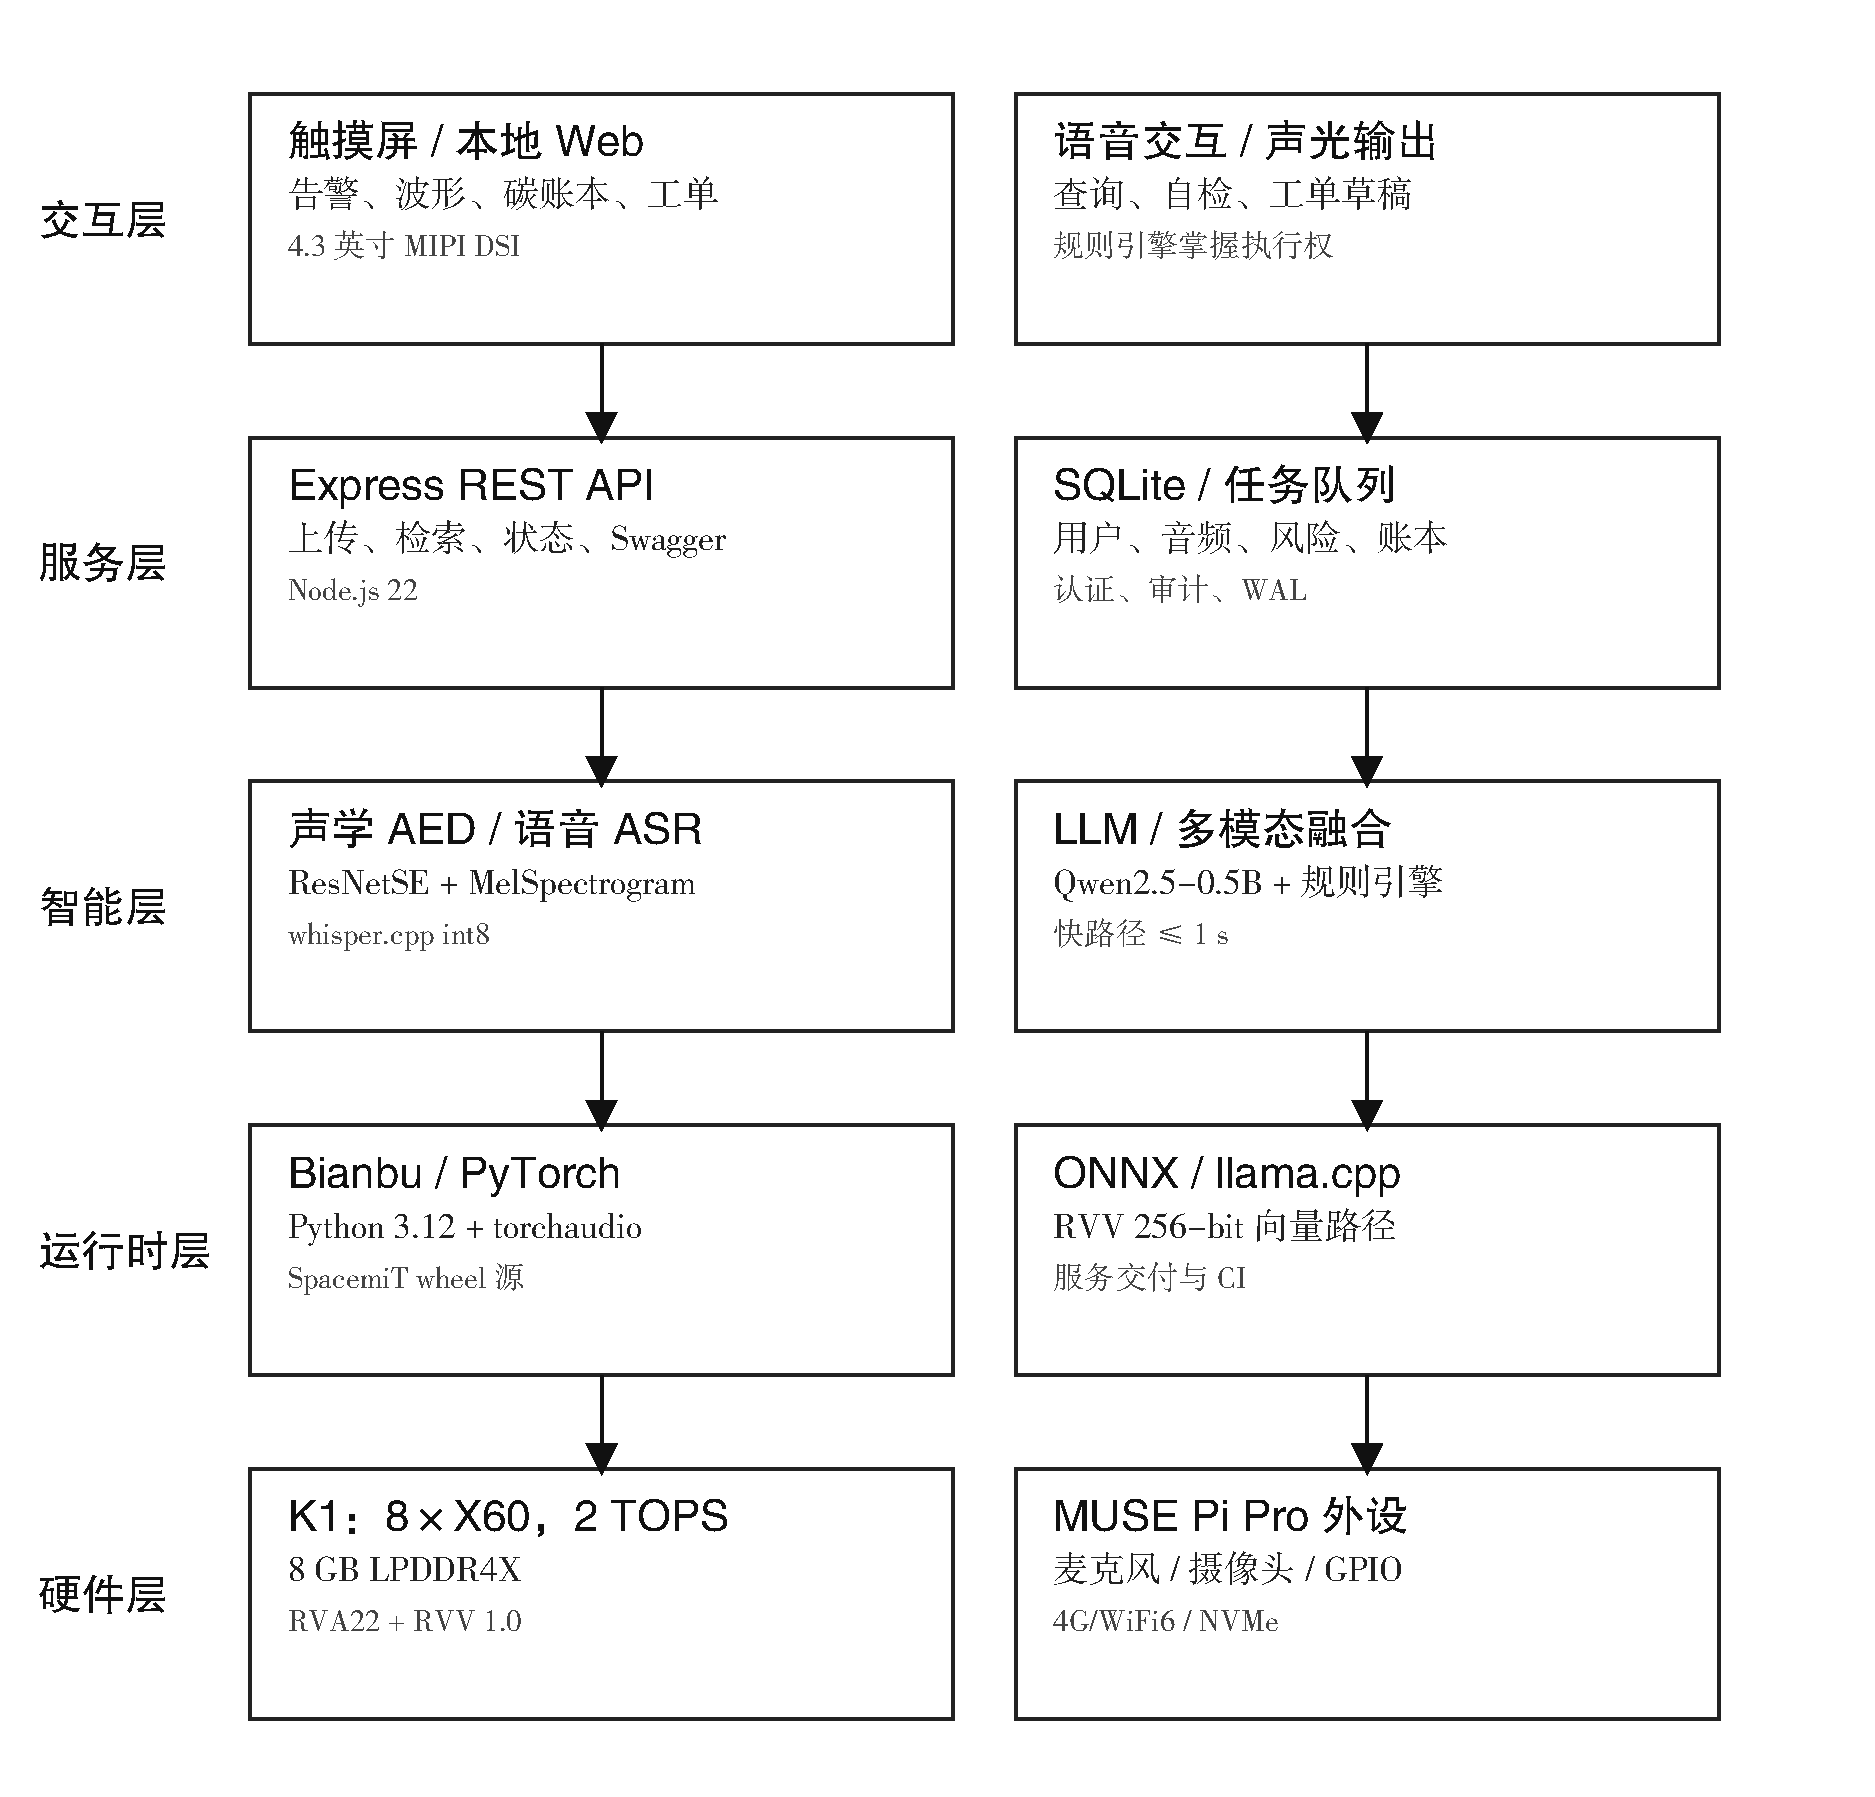
\includegraphics[width=0.96\linewidth]{figures/fig1_architecture.pdf}
  \caption{K1 边缘智能终端总体架构}
  \label{fig:arch}
\end{figure}

\subsection{数据流}

一条完整的漏水事件沿声学链路流动：麦克风或上传音频先被切为 16 kHz、1--4 s 的单声道片段，经 MelSpectrogram（\(80\times400\)）送入 ResNetSE 三分类，得到风险等级与置信度；规则引擎据此触发屏幕告警、工单或碳账本条目，现场复核后归档并回流模型。

语音指令沿交互链路流动：语音经 VAD 截断后送入 whisper.cpp 转写，领域词表与意图解析把文本映射为查询、自检或工单草稿，快路径直接交给规则引擎执行；需要解释或长文本时，异步调用本地 LLM，不阻塞现场动作。

两条路径共享同一份“证据包”：设备 ID、时间、音频片段哈希、模型版本、置信度、规则命中项、操作员确认记录。这样，LLM 生成的工单不会脱离证据，碳账本也可以追溯到具体漏点。

\subsection{部署单元}

当前仓库采用“单容器全栈”部署：Nginx 提供前端静态文件和 \texttt{/api/} 反向代理，Node.js 后端监听 3000，Python 推理脚本由后端调用。生产镜像由 \texttt{Dockerfile.prod.riscv} 构建，基础镜像为 \texttt{harbor.spacemit.com/bianbu/bianbu:latest}，启动脚本 \texttt{start.sh} 同时拉起 Node 和 Nginx。

% =====================================================================
\section{声学感知方法}
\label{sec:acoustic}

\subsection{数据集与标签}

项目使用的本团队私有数据集。数据主要来自人工采集的管道音频，经过筛选后约两千条高质量样本，按风险等级分为三类：高风险 420 条、低风险 518 条、无风险 462 条用于训练/验证，独立测试集分别为 64、79、70 条。训练集与验证集按约 9:1 划分，测试集不参与训练。三类样本数量不完全均衡，训练时通过类别权重和增强缓解。

\subsection{预处理}

推理前的处理流程与训练保持一致：

\begin{enumerate}
  \item 重采样：统一到 16 kHz，单声道。
  \item 时长约束：最短 1 s，最长 4 s；超过 4 s 的音频裁剪，短于 1 s 的拒绝并提示。
  \item 音量归一化：按 RMS 归一化到 \(-20\) dB，降低录音增益差异。
  \item 特征提取：MelSpectrogram，\(n_{\text{fft}}=1024\)、hop length \(=320\)、\(n_{\text{mels}}=80\)、\(f_{\min}=20\) Hz、\(f_{\max}=8000\) Hz。
  \item 张量化：\(1\times80\times400\) 的浮点张量，送入模型。
\end{enumerate}

音量归一化的核心计算为

\begin{equation}
  a' = a \cdot \frac{10^{L_{\text{target}}/20}}
  {\sqrt{\frac{1}{N}\sum_{i=1}^{N}a_i^2}},
  \label{eq:normalize}
\end{equation}

其中 \(a\) 和 \(a'\) 分别为归一化前后的采样序列，\(a_i\) 为第 \(i\) 个采样点，\(N\) 为采样点数，\(L_{\text{target}}\) 为目标声压级（本文取 \(-20\) dB）。归一化后再裁剪到 \([-1,1]\)，避免削波。

\subsection{ResNetSE 模型}

模型主干为 ResNetSE：在残差网络\cite{resnet}中加入 SE 通道注意力\cite{se}。SE 模块分为三步。

\textbf{Squeeze（压缩）}：对每个通道做全局平均池化，得到通道描述向量

\begin{equation}
  z_c = \frac{1}{HW}\sum_{i=1}^{H}\sum_{j=1}^{W}u_c(i,j).
  \label{eq:squeeze}
\end{equation}

其中 \(u_c(i,j)\) 表示第 \(c\) 个通道在空间位置 \((i,j)\) 的激活值，\(H\) 和 \(W\) 分别为特征图的高和宽，\(z_c\) 为通道 \(c\) 的全局统计量。

\textbf{Excitation（激励）}：通过两层全连接学习通道权重

\begin{equation}
  \alpha = \sigma\left(W_2\,\delta\left(W_1 z\right)\right),
  \label{eq:excitation}
\end{equation}

其中 \(z\) 为式\eqref{eq:squeeze}得到的通道统计向量，\(W_1\in\mathbb{R}^{C/r\times C}\) 和 \(W_2\in\mathbb{R}^{C\times C/r}\) 为两层全连接权重，\(C\) 为通道数，\(r=16\) 为缩放比例，\(\delta\) 为 ReLU，\(\sigma\) 为 Sigmoid，\(\alpha\) 为通道权重向量。

\textbf{Scale（重标定）}：把权重乘回原特征图

\begin{equation}
  \tilde{u}_c = \alpha_c \cdot u_c.
  \label{eq:scale}
\end{equation}

其中 \(\tilde{u}_c\) 为重标定后的第 \(c\) 个通道特征，\(\alpha_c\) 为式\eqref{eq:excitation}得到的第 \(c\) 个通道权重，\(u_c\) 为原通道特征。

SE 模块让网络根据输入动态选择重要通道：泄漏声的稳定频带被增强，随机环境噪声被抑制。它只增加少量参数，适合边缘部署。模型输出三类 logits，经 softmax 得到概率

\begin{equation}
  \pi_i = \frac{e^{z_i}}{\sum_{j=1}^{3}e^{z_j}},
  \label{eq:softmax}
\end{equation}

其中 \(z_i\) 为第 \(i\) 类的 logit，\(\pi_i\) 为第 \(i\) 类的 softmax 概率，\(j\) 遍历三个风险类别。

取最大概率对应的标签作为风险等级，最大概率作为置信度。

\subsection{训练配置}

训练配置的主要参数见表\ref{tab:train}。

\begin{table}[H]
\centering
\small
\caption{声学模型训练配置}
\label{tab:train}
\begin{tabular}{p{5cm}p{8cm}}
\toprule
参数 & 值 \\
\midrule
模型 & ResNetSE \\
特征 & MelSpectrogram，80 维 \\
采样率 & 16 kHz \\
音频时长 & 1--4 s \\
批大小 & 32（训练）、16（评估） \\
优化器 & AdamW \\
学习率 & \(5\times10^{-4}\) \\
权重衰减 & \(1\times10^{-5}\) \\
调度器 & WarmupCosineSchedulerLR \\
训练轮数 & 30 \\
混合精度 & 关闭（CPU 推理优先） \\
标签平滑 & 0.02 \\
\bottomrule
\end{tabular}
\end{table}

数据增强包括 SpecAugment（频率/时间掩蔽）、音量扰动和噪声叠加。增强只在训练阶段启用，推理阶段关闭，保证结果的稳定性。

\subsection{推理链路}

\texttt{backend/py/predict.py} 是 Node 后端与 Python 模型之间的桥。它把命令行参数转成 \texttt{MAClsPredictor} 配置，输出 JSON 风险结果，代码见代码\ref{lst:predict}。

\begin{lstlisting}[language=Python,caption={声学推理入口 \texttt{backend/py/predict.py}（节选）},label={lst:predict}]
import sys, json, argparse, functools
from macls.predict import MAClsPredictor
from macls.utils.utils import add_arguments

def main():
    file_path, dir_path = sys.argv[1], sys.argv[2]
    parser = argparse.ArgumentParser(description="智慧水务音频识别")
    add_arg = functools.partial(add_arguments, argparser=parser)
    cfg = dir_path + "/config/resnet_se.yml"
    add_arg("configs", str, cfg, "配置文件")
    add_arg("use_gpu", bool, False, "是否使用GPU预测")
    labels = dir_path + "/dataset/label_list.txt"
    add_arg("overwrites", str,
            "dataset_conf.label_list_path=" + labels,
            "覆盖写入的配置文件参数")
    add_arg("model_path", str, dir_path + "/model/", "模型路径")
    args = parser.parse_args(args=[])
    predictor = MAClsPredictor(
        configs=args.configs, model_path=args.model_path,
        use_gpu=args.use_gpu, overwrites=args.overwrites,
        log_level="error")
    result, score = predictor.predict(file_path)
    result = {"2": "高风险", "1": "无风险"}.get(result, "低风险")
    print(json.dumps({"risk_level": result, "confidence": score}))

main()
\end{lstlisting}

后端上传接口在写入 SQLite 后异步调用该脚本：

\begin{lstlisting}[language=JavaScript,caption={后端异步调用推理脚本（节选）},label={lst:node}]
const options = {
  scriptPath: path.join(__dirname, "py"),
  args: [filePath, path.join(__dirname, "py")],
};
PythonShell.run("predict.py", options).then(results => {
  const prediction = JSON.parse(results[0]);
  const sql = "UPDATE audio_files SET risk_level = ?, confidence = ? " +
              "WHERE id = ?";
  db.run(sql, [prediction.risk_level,
               prediction.confidence, audioFile.id]);
});
\end{lstlisting}

这条链路的优点是简单、可读、容易替换模型；缺点是每次推理都要启动 Python 进程并加载 36.8 MB 模型，冷启动时延高。在本团队的优化实践中，将该流程改为常驻 worker（第\ref{sec:optimization}节），这是 K1 板端达到 1 s 级响应的关键。

\subsection{风险等级与业务动作}

\begin{table}[htbp]
\centering
\small
\caption{风险等级与默认业务动作}
\label{tab:risk}
\begin{tabular}{p{2.4cm}p{4.6cm}p{6.8cm}}
\toprule
模型输出 & 业务含义 & 默认动作 \\
\midrule
高风险 & 泄漏特征明显，置信度高 & 立即屏幕/声光告警；推送工单；安排现场复核 \\
低风险 & 有泄漏迹象但证据强度较低 & 记录并复听；提高采样频率；24 h 内复核 \\
无风险 & 判定为无风险 & 归档；按周期继续监测 \\
\bottomrule
\end{tabular}
\end{table}

置信度低于阈值（默认 0.60）时，不直接告警，转为“待复核”。连续多个时间窗命中高风险时，提升告警等级。规则引擎保留最终决定权，模型只提供证据。

% =====================================================================
\section{多模态交互}
\label{sec:multimodal}

\subsection{为什么需要语音}

阀井和泵房是典型的“双手被占用”场景：巡检人员戴手套、拿手电、扶梯子，掏手机或点屏幕不方便。语音指令可以减少操作步骤，也适合戴安全帽、口罩的现场环境。语音模块按“受限助手”设计：地下泵房有持续机械噪声，ASR 的识别率会下降；开放域语音还会带来误触发和隐私问题。因此本文采用“受限指令集 + 置信度门槛 + 屏幕确认”的方案，语音只触发查询、自检和工单草稿。

\subsection{ASR 命令集与部署}

覆盖高频、低风险指令，见表\ref{tab:asr}。

\begin{table}[H]
\centering
\small
\caption{受限语音指令集}
\label{tab:asr}
\begin{tabular}{p{2.8cm}p{5.4cm}p{6.6cm}}
\toprule
意图 & 示例语句 & 动作 \\
\midrule
查询设备 & “查询三号阀井” & 屏幕显示该设备最近一次风险与时间 \\
开始自检 & “开始自检” & 麦克风、模型、存储、网络逐项检查 \\
生成工单 & “生成工单” & 基于当前证据包生成工单草稿，等待确认 \\
静音告警 & “静音十分钟” & 仅静音本地蜂鸣器，不关闭记录 \\
播放录音 & “播放最近一次” & 播放最近一次高风险音频片段 \\
帮助 & “我该怎么做” & 调用 LLM 或模板，给出处置步骤 \\
\bottomrule
\end{tabular}
\end{table}

在 K1 上，本文选择 whisper.cpp 的 int8 量化路径\cite{whisper}。原因是大模型 ASR 对 2 TOPS 来说太重，而受限指令集不需要通用大模型。\texttt{tiny} 或 \texttt{base} 模型配合 VAD 截断，3 s 语音的识别可以控制在亚秒级。板端编译命令见代码\ref{lst:whisper}。

\begin{lstlisting}[language=bash,caption={whisper.cpp 在 K1 上的编译与量化},label={lst:whisper}]
git clone https://github.com/ggerganov/whisper.cpp
cd whisper.cpp
cmake -B build -DGGML_RVV=ON -DCMAKE_BUILD_TYPE=Release
cmake --build build -j4
./models/download-ggml-model.sh base
./build/bin/quantize models/ggml-base.bin \
  models/ggml-base-q5_1.bin q5_1
\end{lstlisting}

工程上用 Python 把 CLI 文本封装为 JSON。语音先做 VAD，静音不上传；识别结果经过领域词表纠错（设备名、阀井编号、专业术语），再用规则解析意图。置信度低于阈值时，屏幕提示“没听清，请再说一次”，不执行动作。

\subsection{本地大模型}

LLM 在本系统里做三件事：解释、工单和问答。解释是把“高风险、置信度 0.87、连续 3 个窗口命中”翻译成运维人员能理解的语言；工单是根据证据包生成结构化 JSON；问答是基于本地运维手册做检索增强问答。LLM 不做三件事：不直接控制阀门、不替代模型置信度、不在快路径上阻塞现场动作。

选择 Qwen2.5-0.5B-Instruct 的 Q4\_K\_M 量化版本\cite{qwen}，理由是 0.5B 级模型在 8 GB 内存的 K1 上可以常驻，Q4\_K\_M 约 0.4 GB，首 token 时延可控；对于“解释 + 模板化 JSON”这类任务，小模型足够。若板端实测质量低于门槛，可升级到 1B 级模型，但必须重新测量首 token 时延和内存占用。llama.cpp 的启动方式见代码\ref{lst:llama}。

\begin{lstlisting}[language=bash,caption={本地 LLM 启动（llama.cpp）},label={lst:llama}]
./llama-server \
  -m models/qwen2.5-0.5b-instruct-q4_k_m.gguf \
  --host 127.0.0.1 --port 8081 \
  -c 2048 -t 6 --mlock
\end{lstlisting}

LLM 输出“处置意见”，执行由规则引擎完成。执行前做四道检查：Schema 校验、证据引用、动作白名单、人工确认。工具调用的 JSON Schema 示例见代码\ref{lst:schema}。

\begin{lstlisting}[language=JavaScript,caption={工单工具调用的 JSON Schema（设计示例）},label={lst:schema}]
{
  "name": "create_work_order",
  "description": "根据证据包生成工单草稿，不执行任何物理动作",
  "parameters": {
    "type": "object",
    "required": ["evidence_id", "device_id", "risk", "actions", "safety"],
    "properties": {
      "evidence_id": { "type": "string" },
      "device_id":   { "type": "string" },
      "risk":        { "enum": ["high", "low", "none"] },
      "actions":     { "type": "array", "items": { "type": "string" } },
      "safety":      { "type": "array", "items": { "type": "string" } }
    }
  }
}
\end{lstlisting}

\subsection{可选视觉复核}

CV 作为可选复核链路，在高风险场景提供额外证据：摄像头拍一张阀井照片，识别积水、管壁锈蚀、表计读数或异物遮挡，作为声学证据的补充。实现上选择轻量检测/分类模型（如 YOLOv8n、PP-PicoDet 或 MobileNetV3），导出 ONNX，用 ONNX Runtime 的 CPU EP 在 K1 上推理。CV 的触发条件是“声学高风险且摄像头可用”，避免持续视频推理抢占 CPU。图片在本地做隐私模糊（人脸、车牌、门牌），只保留设备区域。CV 输出同样只作为证据，不单独触发控制。

\subsection{快慢双路径}

多模态融合的难点是确定“谁有最终决定权”。本文把 LLM 放在慢路径，把规则引擎放在快路径，如图\ref{fig:pipeline}所示；快路径保证交互时延，慢路径承担解释、工单与碳账本，两者共享同一份证据包。

\begin{figure}[ht]
  \centering
  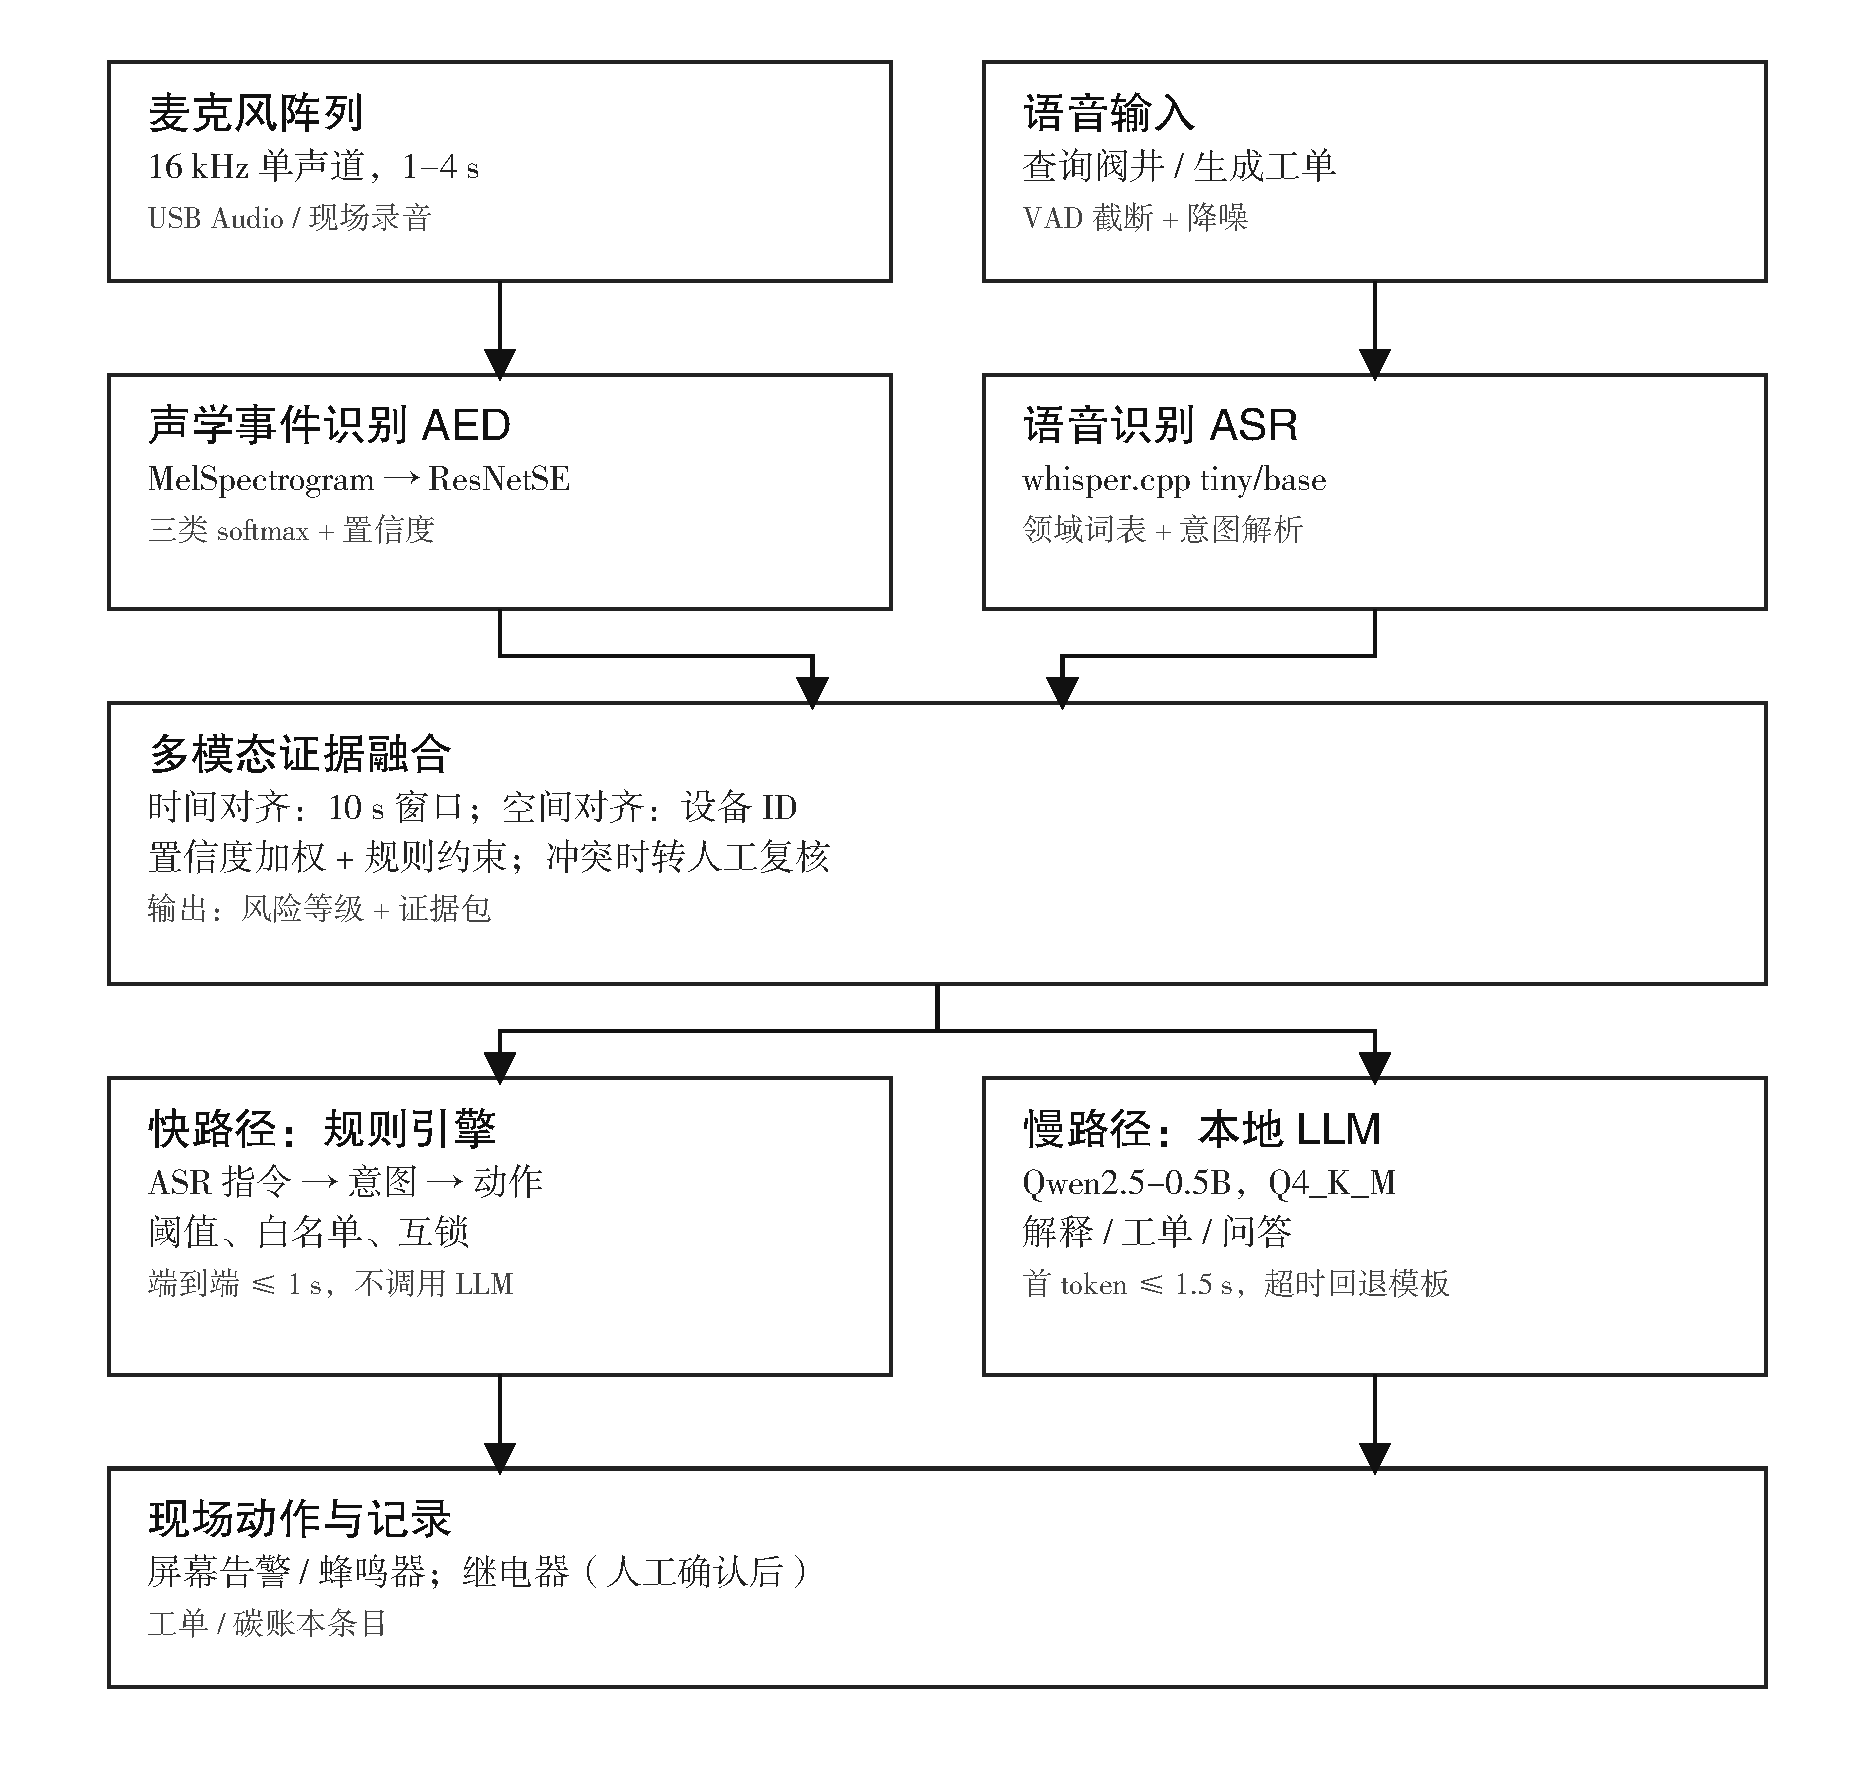
\includegraphics[width=0.96\linewidth]{figures/fig2_pipeline.pdf}
  \caption{快慢双路径多模态推理流水线}
  \label{fig:pipeline}
\end{figure}

\begin{table}[ht]
\centering
\small
\caption{多模态融合状态机}
\label{tab:fusion}
\begin{tabular}{p{2.4cm}p{4.4cm}p{3.0cm}p{3.8cm}}
\toprule
状态 & 输入 & 判断 & 输出 \\
\midrule
监听 & 麦克风 1--4 s 窗口 & 能量/噪声门限 & 进入识别或丢弃 \\
声学识别 & 音频窗口 & ResNetSE 三类概率 & 风险 + 置信度 \\
语音识别 & VAD 截断的语音 & whisper.cpp + 意图解析 & 指令 + 槽位 \\
融合 & 声学/语音/视觉证据 & 时间、设备、置信度对齐 & 证据包 \\
快路径 & 指令/高风险事件 & 规则、阈值、白名单 & 屏幕/声光/工单 \\
慢路径 & 证据包 & LLM 解释/工单/问答 & 文本 + JSON \\
复核 & 人工确认 & 现场照片、听音 & 归档/误报回流 \\
\bottomrule
\end{tabular}
\end{table}

快路径的时延预算为：音频解码与重采样 50 ms、Mel 特征 30 ms、ResNetSE 80--150 ms、规则/意图 20 ms、屏幕/继电器 20 ms，合计不超过 1 s。LLM 不在快路径上，首 token 目标为 1.5 s，完整工单目标为 8 s；超时自动回退模板。

% =====================================================================
\section{RISC-V 深度学习运行时适配}
\label{sec:riscv}

\subsection{难点}

把 PyTorch 模型放到 RISC-V 上，难点集中在运行时：

\begin{itemize}
  \item \textbf{wheel 来源}：PyPI 上的 \texttt{torch} 轮子主要面向 x86\_64 和 aarch64，RISC-V 需要专门的构建源。
  \item \textbf{ABI 一致性}：\texttt{torch}、\texttt{torchvision}、\texttt{torchaudio}、\texttt{numpy}、\texttt{av} 必须来自同一套编译环境，混用会出现符号未定义或段错误。
  \item \textbf{音频前端}：\texttt{librosa} 依赖 \texttt{numba} JIT，\texttt{numba} 对 RISC-V 支持有限；\texttt{scipy} 的编译扩展在 RISC-V 上构建时间长、依赖 BLAS/LAPACK。
  \item \textbf{动态库路径}：\texttt{libtorch}、\texttt{libgomp}、\texttt{libsleef}、\texttt{libstdc++} 的搜索路径需要显式配置。
  \item \textbf{系统差异}：Bianbu 的 Python 版本、glibc、OpenMP 版本与通用 Ubuntu 镜像存在差异，安装脚本需要针对 Bianbu 单独适配。
\end{itemize}

\subsection{适配栈}

团队采用的基线见表\ref{tab:stack}，分层关系如图\ref{fig:stack}所示。

\begin{table}[H]
\centering
\small
\caption{RISC-V 深度学习运行时基线}
\label{tab:stack}
\begin{tabular}{p{3.2cm}p{5.4cm}p{5.8cm}}
\toprule
组件 & 版本/来源 & 说明 \\
\midrule
基础镜像 & \path{harbor.spacemit.com/bianbu/bianbu:latest} & 进迭时空 Bianbu 系统 \\
Python & 3.12 & 系统自带，避免自编译 Python \\
PyTorch & 2.8.0 & 进迭时空 PyPI 源 \\
torchvision & 0.23.0 & 与 torch 配套 \\
torchaudio & 2.8.0 & 与 torch 配套，提供重采样/卷积 \\
av & 11.0.0 & 音视频解码依赖 \\
numba & 0.62.1 & 固定版本，避免与 llvmlite 不匹配 \\
llvmlite & 0.43.0 & 与 numba 配套 \\
Node.js & 22 & 后端与前端构建 \\
\bottomrule
\end{tabular}
\end{table}

\begin{figure}[ht]
  \centering
  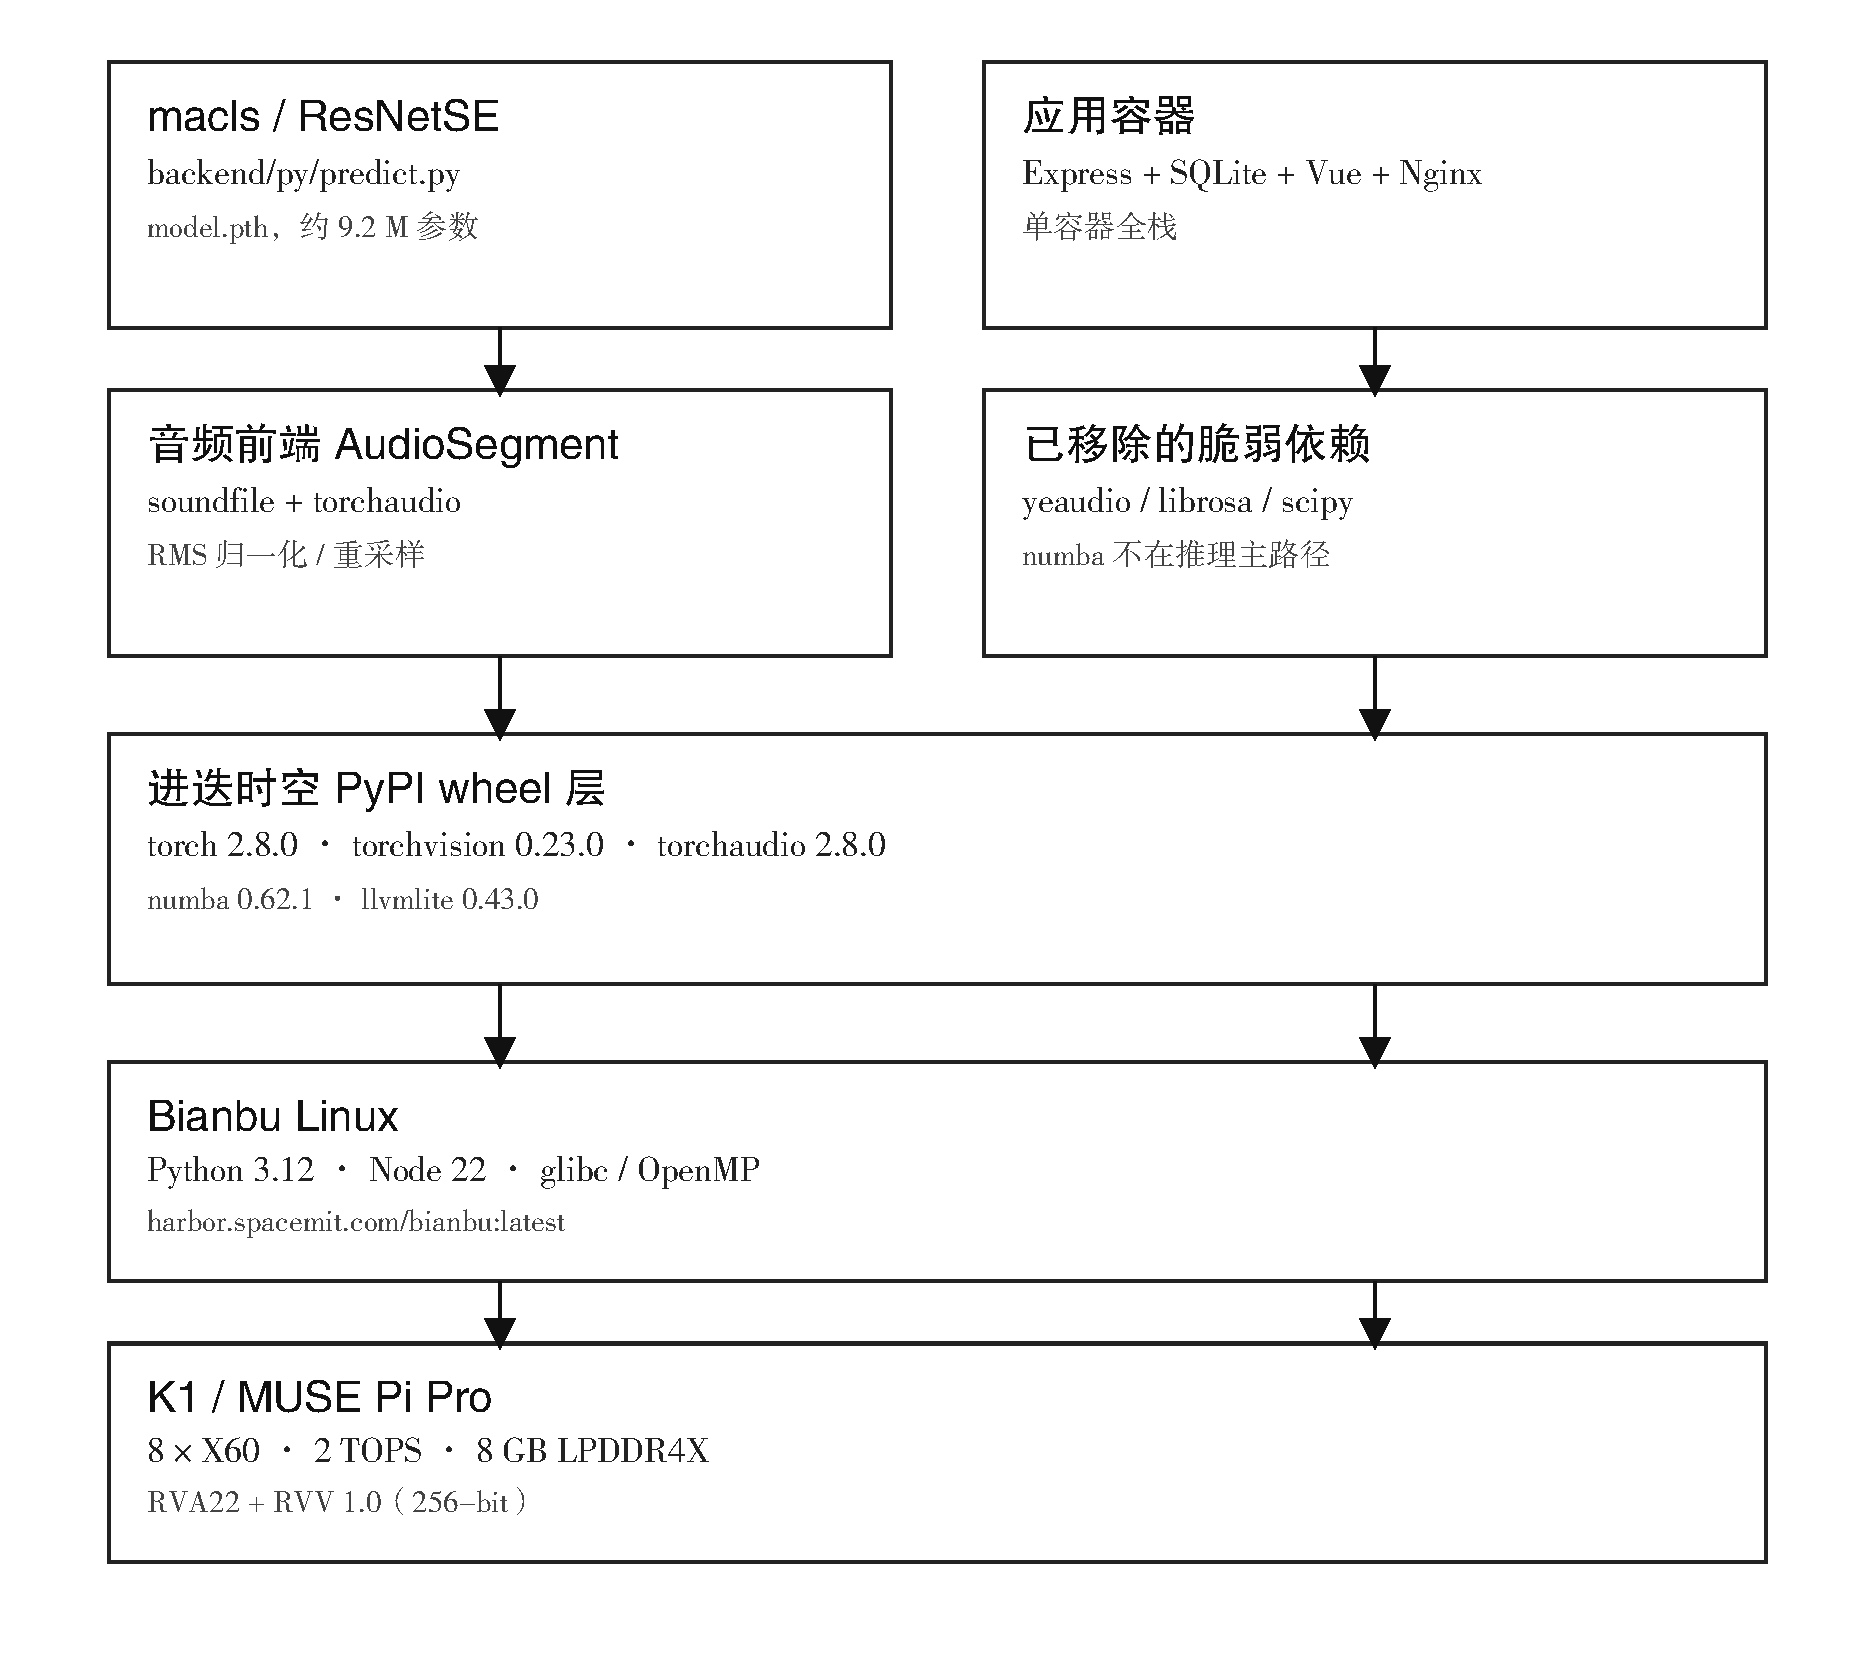
\includegraphics[width=0.96\linewidth]{figures/fig3_riscv_stack.pdf}
  \caption{RISC-V 深度学习运行时适配栈}
  \label{fig:stack}
\end{figure}

所有架构相关的二进制都从进迭时空 wheel 源安装，不使用 \texttt{pip install torch} 的默认源，避免复杂的系统依赖冲突问题。

\subsection{Dockerfile 与 ABI 绑定}

\texttt{Dockerfile.prod.riscv} 把版本、源、动态库路径和构建顺序固定下来，关键片段见代码\ref{lst:docker}。

\begin{lstlisting}[language=bash,caption={RISC-V 生产镜像关键片段 \texttt{Dockerfile.prod.riscv}},label={lst:docker}]
FROM harbor.spacemit.com/bianbu/bianbu:latest
SHELL ["/bin/bash", "-c"]

ENV PYTHONHTTPSVERIFY=0
ENV LD_LIBRARY_PATH="/usr/local/lib/python3.12/dist-packages/torch/lib:${LD_LIBRARY_PATH}"

RUN apt-get update && apt-get install -y \
    nginx curl bash wget nodejs npm python3-pip python3-full \
    build-essential cmake libopenblas-dev libjpeg-dev zlib1g-dev \
    libsleef3 libomp5 libnuma1 libsndfile1 libavformat60 ffmpeg

RUN pip config set global.extra-index-url \
    https://git.spacemit.com/api/v4/projects/33/packages/pypi/simple

RUN pip install --index-url \
    https://git.spacemit.com/api/v4/projects/33/packages/pypi/simple \
    --trusted-host git.spacemit.com \
    torch==2.8.0 torchvision==0.23.0 torchaudio==2.8.0 \
    av==11.0.0 numba==0.62.1 llvmlite==0.43.0 \
    --break-system-packages

RUN pip install ./whl/AudioClassification-Pytorch/ --break-system-packages
\end{lstlisting}

几个容易忽略的细节：\texttt{LD\_LIBRARY\_PATH} 指向 \texttt{torch/lib}，保证 \texttt{libtorch\_cpu.so} 能加载 \texttt{libgomp}/\texttt{libsleef}；先装系统库（\texttt{libsndfile1}、\texttt{libavformat60}、\texttt{libomp5}），再装 Python 包，保证运行期 \texttt{.so} 完整；固定 \texttt{numba==0.62.1} 与 \texttt{llvmlite==0.43.0}，让 pip 解析到兼容组合；\texttt{--break-system-packages} 是 Bianbu 系统 Python 的限制，在虚拟环境中应去掉。

\subsection{音频前端替换}

原项目使用 \texttt{yeaudio} 的 \texttt{AudioSegment}，RISC-V 上的稳定 wheel 供给有限。团队把音频前端替换为 \texttt{torchaudio + soundfile}，保持原有 API 不变，核心实现见代码\ref{lst:audio}，文件路径为 \path{whl/AudioClassification-Pytorch/macls/data_utils/augmentation.py}。这份实现的价值在于：读取用 \texttt{soundfile}，绕开 \texttt{torchaudio} 新版本对 \texttt{torchcodec} 的依赖；重采样用 \path{torchaudio.transforms.Resample}，走 PyTorch 的张量路径，和模型在同一套运行时里；音量归一化用 NumPy 的 RMS，计算量小，与 \texttt{librosa}/\texttt{scipy} 解耦；API 与原来的 \texttt{AudioSegment} 保持一致，训练和推理代码的改动集中在音频前端。数据增强中的时间拉伸、混响等操作也改为 \path{torchaudio.functional.speed} 和 \path{torchaudio.functional.convolve}。这一步把 \texttt{numba} 从推理主路径上移除，显著降低了 RISC-V 上的不确定性。

\begin{lstlisting}[language=Python,caption={RISC-V 友好的 \texttt{AudioSegment} 实现（节选）},label={lst:audio}]
import numpy as np
import torch
import torchaudio
import soundfile as sf

class AudioSegment:
    def __init__(self, samples, sample_rate):
        if isinstance(samples, torch.Tensor):
            self.samples = samples.cpu().numpy().astype(np.float32)
        else:
            self.samples = np.asarray(samples, dtype=np.float32)
        self.sample_rate = sample_rate

    @classmethod
    def from_file(cls, path):
        samples, sr = sf.read(path, dtype="float32")
        if samples.ndim > 1:
            samples = np.mean(samples, axis=1)
        return cls(samples, sr)

    def resample(self, target_sr):
        if target_sr == self.sample_rate:
            return
        wav = torch.from_numpy(self.samples).unsqueeze(0)
        rs = torchaudio.transforms.Resample(
            orig_freq=self.sample_rate, new_freq=target_sr)
        self.samples = rs(wav).squeeze(0).numpy().astype(np.float32)
        self.sample_rate = target_sr

    def normalize(self, target_db=-20):
        rms = np.sqrt(np.mean(self.samples ** 2))
        if rms == 0 or np.isnan(rms):
            return
        target_rms = 10 ** (target_db / 20.0)
        self.samples = np.clip(
            self.samples * (target_rms / rms), -1.0, 1.0)
\end{lstlisting}

\subsection{构建与交付}

RISC-V 镜像通过 GitHub Actions 的 QEMU + Buildx 交叉构建，推送到 GHCR。本地构建命令为

\begin{lstlisting}[language=bash,caption={RISC-V 镜像构建命令},label={lst:build}]
./build-and-push.sh --build-only -t latest-riscv
# 或构建并推送
export GITHUB_TOKEN=ghp_xxx
./build-and-push.sh --push -t latest-riscv -v 1.0.0
\end{lstlisting}

CI 工作流 \path{.github/workflows/docker-image-riscv.yml} 负责：在 x86 runner 上构建前端 \path{frontend/dist}；设置 QEMU binfmt 与 Buildx；使用 \path{Dockerfile.prod.riscv} 构建 \texttt{linux/riscv64} 镜像；注入 \texttt{BUILD\_TIME}、\texttt{VERSION}、\texttt{GIT\_COMMIT}；推送到 \path{ghcr.io/lvshujun0918/ai_water-riscv}，标签包含 \texttt{latest-riscv} 和 \texttt{riscv64-<sha>}。

QEMU 构建验证镜像可构建、依赖可安装；本文另用 QEMU 用户态模拟验证推理链路，时延只作参考，最终性能与功耗以 MUSE Pi Pro 实测为准。

\subsection{适配中的难点问题}

\begin{table}[H]
\centering
\small
\caption{RISC-V 适配常见问题与处理}
\label{tab:pitfalls}
\begin{tabular}{p{4.4cm}p{4.6cm}p{5.0cm}}
\toprule
现象 & 根因 & 处理 \\
\midrule
\texttt{import torch} 报符号未定义 & torch 与 torchaudio/torchvision 来自不同构建 & 全部从同一 SpacemiT 源、同一批次安装 \\
\texttt{libgomp.so.1} 找不到 & 动态库路径未包含 torch/lib & 设置 \texttt{LD\_LIBRARY\_PATH} \\
\texttt{numba} 导入失败 & numba/llvmlite 版本不匹配 & 固定 0.62.1 / 0.43.0 \\
\texttt{librosa} 加载慢或超时 & 依赖 numba JIT、soundfile 后端 & 推理路径改用 torchaudio + soundfile \\
\texttt{scipy} 构建超过 1 小时 & RISC-V 预编译 wheel 供给有限 & 不在板端编译；镜像构建阶段使用预编译依赖 \\
torchaudio 报后端错误 & 新版本默认依赖 torchcodec & 音频读取用 soundfile，重采样用 torchaudio \\
容器内权限错误 & 非 root 用户写权限需配置 & 构建时创建目录并 \texttt{chown 1000:1000} \\
前端请求 404 & Nginx 代理路径需与 API 前缀对齐 & \texttt{/api/} 反代到 \texttt{localhost:3000/api/} \\
\bottomrule
\end{tabular}
\end{table}

% =====================================================================
\section{性能优化}
\label{sec:optimization}

\subsection{指标定义}

本文定义：

\begin{table}[H]
\centering
\small
\caption{性能指标与测量口径}
\label{tab:metrics}
\begin{tabular}{p{3.2cm}p{3.4cm}p{3.4cm}p{4.0cm}}
\toprule
指标 & 起点 & 终点 & 说明 \\
\midrule
声学单窗时延 & 音频张量进入模型 & 输出三类概率 & 不含音频读取/解码 \\
端到端声学时延 & 上传完成 & 数据库写入风险 & 含解码、特征、推理、写库 \\
ASR 时延 & 语音结束 & 文本返回 & 3 s 语音，含 VAD \\
快路径时延 & 语音结束 & 屏幕/继电器响应 & ASR + 意图 + 规则 \\
LLM 首 token & 请求发出 & 第一个 token & 2048 上下文，Q4\_K\_M \\
冷启动 & 进程启动 & 模型可推理 & 含 Python 导入、权重加载 \\
内存 & 稳定运行 10 min & RSS & 不含页缓存 \\
功耗 & 稳定负载 & 整机输入功率 & USB PD 功率计 \\
\bottomrule
\end{tabular}
\end{table}

所有时延报告 p50 和 p95，预热 10 次，连续 30 次；冷启动单独统计，不混入热推理。

\subsection{常驻推理 worker}

改造方案：后端启动时拉起一个常驻 Python worker，模型只加载一次；Node 通过本地 HTTP 或 Unix socket 发送音频路径/字节，worker 返回 JSON，见代码\ref{lst:worker}。

\begin{lstlisting}[language=Python,caption={常驻推理 worker（设计示例）},label={lst:worker}]
import json, os
from http.server import BaseHTTPRequestHandler, HTTPServer
from macls.predict import MAClsPredictor

BASE = os.path.dirname(os.path.abspath(__file__))
predictor = MAClsPredictor(
    configs=os.path.join(BASE, "config/resnet_se.yml"),
    model_path=os.path.join(BASE, "model"),
    use_gpu=False,
    overwrites=f"dataset_conf.label_list_path={BASE}/dataset/label_list.txt",
    log_level="error")

class Handler(BaseHTTPRequestHandler):
    def do_POST(self):
        n = int(self.headers.get("Content-Length", 0))
        payload = json.loads(self.rfile.read(n))
        label, score = predictor.predict(payload["path"])
        body = json.dumps({
            "risk_level": {"2": "高风险", "1": "无风险"}.get(label, "低风险"),
            "confidence": score}).encode()
        self.send_response(200)
        self.send_header("Content-Type", "application/json")
        self.send_header("Content-Length", str(len(body)))
        self.end_headers()
        self.wfile.write(body)

    def log_message(self, *args):
        pass

if __name__ == "__main__":
    HTTPServer(("127.0.0.1", 5001), Handler).serve_forever()
\end{lstlisting}

这个改动把“模型加载”从每次请求移到进程启动，热推理只做解码、特征和一次前向。代价是常驻内存增加（约 300--500 MB，取决于 PyTorch 运行时），对 8 GB 的 K1 可以接受。worker 需要看门狗：健康检查失败时重启，重启期间请求排队或降级。

\subsection{模型侧优化}

推理输入固定为 \(1\times1\times80\times400\)，不使用动态轴。固定形状让 ONNX Runtime 可以预分配内存、融合算子，也避免每次推理重新推导形状。导出 ONNX 的伪代码为：

\begin{lstlisting}[language=Python,caption={固定形状 ONNX 导出},label={lst:onnx}]
import torch
model.load_state_dict(torch.load("model/model.pth", map_location="cpu"))
model.eval()
dummy = torch.randn(1, 1, 80, 400)
torch.onnx.export(
    model, dummy, "resnetse_fixed.onnx",
    opset_version=17,
    input_names=["mel"], output_names=["logits"],
    dynamic_axes=None)
\end{lstlisting}

INT8 量化采用训练后静态量化（PTQ），校准集从训练集随机抽取 200 条，覆盖三类和不同噪声水平。权重采用 per-channel 对称量化，激活采用 per-tensor 非对称量化，校准方法为 percentile 99.99\%，格式为 QDQ。验收标准是量化后准确率相对 FP32 下降不超过 1 个百分点；若超过，改用 QAT 或保留 SE 模块的 FP32 分支。量化精度受校准集覆盖影响：声学模型的输入是连续的 Mel 频谱，低幅值噪声容易被量化误差淹没，因此校准集需要包含无风险样本和低信噪比样本。

如果 INT8 后仍然超时，可以按通道重要性剪枝 10--20\%，再用原模型蒸馏恢复精度。剪枝对 ResNetSE 的残差结构要小心：保留 shortcut 通道，训练才稳定。量化和剪枝的次序放在第\ref{sec:future}节展开。

\subsection{运行时与系统优化}

\begin{table}[H]
\centering
\small
\caption{运行时与系统优化项}
\label{tab:runtime}
\begin{tabular}{p{3.6cm}p{6.2cm}p{4.6cm}}
\toprule
优化项 & 做法 & 预期收益 \\
\midrule
ONNX Runtime 图优化 & \texttt{ORT\_ENABLE\_ALL} & 算子融合、常量折叠 \\
线程数 & \texttt{intra\_op=6}、\texttt{inter\_op=1} & 留 2 核给 ASR/UI，避免过度订阅 \\
内存池 & 开启 CPU arena & 减少分配抖动 \\
执行模式 & 顺序执行 & 单请求低时延 \\
数据布局 & NCHW，连续内存 & 向量化友好 \\
RVV & 使用支持 RVV 的算子库 & 256-bit 向量加速 \\
页缓存 & 模型常驻，\texttt{mlock}（LLM） & 避免首次加载抖动 \\
绑核 & 推理线程绑定 4--6 个核 & 降低迁移开销 \\
SQLite & \texttt{PRAGMA journal\_mode=WAL} & 减少读写锁冲突 \\
预热 & 开机空推理一次 & 触发算子初始化 \\
超时降级 & 推理超过 2 s 返回“处理中” & 避免 HTTP 悬挂 \\
看门狗 & systemd \texttt{Restart=always} & worker 异常自动重启 \\
\bottomrule
\end{tabular}
\end{table}

K1 的 8 个 X60 核是同构的，不需要大小核调度；但 ASR、LLM、Web 服务会争抢 CPU。部署时用 cgroup 或 \texttt{taskset} 给推理 worker 留出稳定核数，避免 Web 请求把推理线程挤走。LLM 使用 Q4\_K\_M 量化、2048 上下文、\texttt{-t 6}、\texttt{--mlock}，温度 0.2，\texttt{max\_tokens=512}，失败/超时回退模板。ASR 先做 VAD，5 s 窗口，\texttt{tiny}/\texttt{base} + int8/q5\_1，领域词表纠错，置信度低于阈值时要求重说。

\subsection{性能预算}

表\ref{tab:budget}给出快路径的设计目标。

\begin{table}[H]
\centering
\small
\caption{快路径时延预算}
\label{tab:budget}
\begin{tabular}{p{5.2cm}p{3.8cm}p{5.4cm}}
\toprule
环节 & 预算 & 备注 \\
\midrule
音频解码 + 重采样 & 50 ms & 16 kHz 单声道，4 s \\
Mel 特征 & 30 ms & \(80\times400\) \\
ResNetSE FP32 & 150 ms & 6 线程 \\
ResNetSE INT8 & 80 ms & 目标，待实测 \\
ASR 3 s 语音 & 800 ms & whisper.cpp base int8 \\
规则/意图 & 20 ms & 本地内存 \\
屏幕/继电器 & 20 ms & GPIO/前端 \\
\midrule
快路径合计 & \(\leq 1\) s & 不含人工确认 \\
\bottomrule
\end{tabular}
\end{table}

% =====================================================================
\section{绿碳效益评估}
\label{sec:carbon}

\subsection{核算边界}

本文的碳账本只覆盖运行阶段：漏损水量、供水电耗、电力碳排、终端自身碳排。边界覆盖漏损水量、供水电耗、电力碳排和终端自身碳排；管网建设、设备制造、化学药剂、维护车辆和人员通勤由单独的清单数据核算。完整 LCA 需要这些数据，本文将运行阶段减排与全生命周期碳中和分开报告。

\subsection{公式}

\begin{equation}
  W_{\text{saved}} = Q_{\text{leak}} \times \Delta t,
  \label{eq:water}
\end{equation}

其中 \(W_{\text{saved}}\) 表示节水量，\(Q_{\text{leak}}\) 表示漏点平均流量，\(\Delta t\) 表示提前发现时间。

\begin{equation}
  E_{\text{saved}} = W_{\text{saved}} \times e_{\text{water}},
  \label{eq:energy}
\end{equation}

其中 \(E_{\text{saved}}\) 表示节电量，\(e_{\text{water}}\) 表示供水综合电耗；\(W_{\text{saved}}\) 已由式\eqref{eq:water}定义。

\begin{equation}
  C_{\text{saved}} = E_{\text{saved}} \times EF,
  \label{eq:carbon}
\end{equation}

其中 \(C_{\text{saved}}\) 表示减排量，\(EF\) 表示电力排放因子；\(E_{\text{saved}}\) 已由式\eqref{eq:energy}定义。

\begin{equation}
  C_{\text{dev}} = P_{\text{dev}} \times t \times EF,
  \label{eq:device}
\end{equation}

其中 \(C_{\text{dev}}\) 表示终端自身碳排，\(P_{\text{dev}}\) 表示终端功率，\(t\) 表示年运行小时；\(EF\) 已由式\eqref{eq:carbon}定义。

\begin{equation}
  C_{\text{net}} = C_{\text{saved}} - C_{\text{dev}}.
  \label{eq:net}
\end{equation}

其中 \(C_{\text{net}}\) 表示净减排量；\(C_{\text{saved}}\) 与 \(C_{\text{dev}}\) 已分别由式\eqref{eq:carbon}和式\eqref{eq:device}定义。本文取 \(EF=0.5366\) kgCO\(_2\)/kWh，来源为生态环境部与国家统计局发布的 2022 年全国电力平均二氧化碳排放因子\cite{mee}；取 \(e_{\text{water}}=0.3\) kWh/m\(^3\) 作为基准，敏感性分析取 0.2--0.5；终端典型功率取 5 W，峰值 10 W。

\subsection{情景计算}

以下数值代入沿用式\eqref{eq:water}--\eqref{eq:net}的符号，不再重复解释。

\textbf{情景 A：单个漏点，0.3 m\(^3\)/h，提前 27 天。} 将 \(Q_{\text{leak}}=0.3\ \text{m}^3/\text{h}\)、\(\Delta t=27\times24\ \text{h}\) 代入式\eqref{eq:water}，得

\begin{equation}
  W_{\text{saved}} = 0.3 \times 24 \times 27 = 194.4\ \text{m}^3,
\end{equation}
\begin{equation}
  E_{\text{saved}} = 194.4 \times 0.3 = 58.3\ \text{kWh},
\end{equation}
\begin{equation}
  C_{\text{saved}} = 58.3 \times 0.5366 = 31.3\ \text{kgCO}_2.
\end{equation}

终端自身年碳排为

\begin{equation}
  C_{\text{dev}} = 0.005 \times 8760 \times 0.5366 = 23.5\ \text{kgCO}_2,
\end{equation}

净减排约 7.8 kgCO\(_2\)/年。这个数字不大，但已经为正；如果算上减少的水处理药剂、泵组磨损和爆管风险，实际收益更高。

\textbf{情景 B：单个漏点，1.0 m\(^3\)/h，提前 27 天。} 节水量 648 m\(^3\)，节电量 194.4 kWh，减排 104.3 kgCO\(_2\)，净减排约 80.8 kgCO\(_2\)/年。

\textbf{情景 C：100 台终端，每台每年发现 1 个 1.0 m\(^3\)/h 漏点。} 节水量 64,800 m\(^3\)/年，节电量 19,440 kWh/年，减排 10.43 tCO\(_2\)/年，终端自身碳排 2.35 tCO\(_2\)/年，净减排约 8.08 tCO\(_2\)/年。

这一量级适合按节点逐步推广。对于供水企业，水费和电费的节省通常比碳收益更直接；碳账本把“漏损控制”纳入 ESG 披露和绿色融资的语言体系。

\subsection{敏感性分析}

表\ref{tab:sensitivity}给出单漏点 1.0 m\(^3\)/h、提前 27 天、扣除终端 23.5 kgCO\(_2\) 后的年减排随综合电耗的变化。

\begin{table}[H]
\centering
\small
\caption{供水综合电耗对单漏点年减排的影响}
\label{tab:sensitivity}
\begin{tabular}{p{4.2cm}p{4.6cm}p{4.6cm}}
\toprule
综合电耗（kWh/m\(^3\)） & 减排（kgCO\(_2\)） & 扣除终端 23.5 kg 后净减排 \\
\midrule
0.2 & 69.5 & 46.0 \\
0.3 & 104.3 & 80.8 \\
0.5 & 173.8 & 150.3 \\
\bottomrule
\end{tabular}
\end{table}

% =====================================================================
\section{部署与实验设计}
\label{sec:evaluation}

\subsection{部署方式}

RISC-V 板端一键部署：

\begin{lstlisting}[language=bash,caption={RISC-V 板端一键部署},label={lst:deploy}]
curl -sSL https://raw.githubusercontent.com/Lvshujun0918/AI_Water/refs/heads/main/install-riscv.sh | bash
\end{lstlisting}

脚本会检查 Docker/Compose、创建 \texttt{uploads} 和 \texttt{db} 目录、下载 \path{docker-compose.riscv.yml}、拉取 GHCR 镜像并启动。启动后在浏览器访问板端 8080 端口，首次进入初始化管理员账户。手动方式为

\begin{lstlisting}[language=bash,caption={手动启动},label={lst:compose}]
git clone https://github.com/Lvshujun0918/AI_Water
cd AI_Water
docker compose -f docker-compose.riscv.yml up -d
\end{lstlisting}

数据持久化：\path{uploads/} 保存上传的音频与证据片段；\path{db/} 保存 SQLite 数据库（用户、音频记录、风险结果、碳账本）。

\subsection{API 与数据模型}

系统 API 包括：
\begin{itemize}[leftmargin=1.6em,itemsep=0pt,topsep=0.2em]
  \item 初始化与认证：\path{/api/init-status}、\path{/api/init-admin}、\path{/api/login}、\path{/api/auth/refresh}；
  \item 用户：\path{/api/users}、\path{/api/users/profile}、\path{/api/users/change-password}；
  \item 音频：\path{/api/audio-files}、\path{/api/audio-files/:id}、\path{/api/upload-audio}、\path{/api/audio-processing-status/:name}；
  \item 自检：\path{/api/test}；Swagger UI 在 \path{/api-docs}。
\end{itemize}

核心表为 \texttt{users} 与 \texttt{audio\_files}。同时在数据库中我们创新性地引入了碳账本，把“漏点—水量—电—碳”的假设和结果固定下来：

\begin{lstlisting}[language=SQL,caption={碳账本表结构},label={lst:ledger}]
CREATE TABLE IF NOT EXISTS carbon_ledger (
  id INTEGER PRIMARY KEY AUTOINCREMENT,
  audio_id INTEGER NOT NULL,
  device_id TEXT,
  leak_flow_m3h REAL,
  saved_hours REAL,
  water_saved_m3 REAL,
  energy_saved_kwh REAL,
  co2_saved_kg REAL,
  grid_factor_kg_per_kwh REAL,
  created_at DATETIME DEFAULT CURRENT_TIMESTAMP,
  FOREIGN KEY (audio_id) REFERENCES audio_files(id)
);
\end{lstlisting}

这张表让碳账本可审计：每个数字都能追溯到公式、输入和排放因子版本。

\subsection{测试环境与指标}

目标测试环境为 MUSE Pi Pro（K1，8 GB LPDDR4X，64 GB eMMC），Bianbu Linux，Python 3.12，PyTorch 2.8.0，torchaudio 2.8.0。音频为 16 kHz 单声道 1--4 s。时延按第\ref{sec:optimization}节定义，预热 10 次、连续 30 次，报告 p50/p95；冷启动单独统计。准确率使用未参与训练的独立测试集，固定随机种子，不调阈值，报告准确率、每类精确率/召回率/F1、混淆矩阵、高风险漏报率和量化前后对比。资源与功耗记录 CPU、RSS、AI 算力占用、整机功率和温度。

AMD64侧配置为 Ryzen 7 PRO 8845HS，Python 3.11.2，PyTorch 2.8.0+cpu；任务绑定 0--7 核并提高调度优先级，输入为 4 s、16 kHz 单声道合成噪声，预热 10 次后连续运行 100 次。该组数据验证模型加载、音频读取、特征提取、前向计算和 \texttt{predict.py} 的 JSON 输出；合成噪声只用于时延，不用于准确率。

\begin{table}[htbp]
\centering
\small
\caption{AMD64 架构模型基线与线程扩展}
\label{tab:devbaseline}
\begin{tabular}{p{3.4cm}p{3.4cm}p{7.0cm}}
\toprule
项目 & 实测值 & 说明 \\
\midrule
模型参数量 & 9,124,475 & ResNetSE，FP32 \\
权重文件 & 36,786,581 B & 约 35.1 MiB \\
模型加载 & 94.5 ms & 进程内加载，6 线程 \\
首窗推理 & 50.4 ms & 含读取、特征与一次前向 \\
热推理 p50/p95 & 30.3 / 34.9 ms & 100 次，6 线程 \\
线程扩展 p50 & 84.8 / 54.3 / 37.8 / 30.3 / 30.1 ms & 1 / 2 / 4 / 6 / 8 线程，各 100 次 \\
\texttt{predict.py} 输出 & 低风险，0.56815 & 链路正常 \\
\bottomrule
\end{tabular}
\end{table}

RISC-V 侧用进迭时空 K1 开发板完成可执行验证及性能测试。

\begin{table}[htbp]
\centering
\small
\caption{RISC-V 环境测试记录}
\label{tab:results}
\begin{tabular}{p{3.6cm}p{5.2cm}p{6.0cm}}
\toprule
项目 & 结果 & 说明 \\
\midrule
运行架构 & \texttt{riscv64} & \texttt{uname -m} \\
Python / PyTorch & 3.12.3 / 2.8.0+spacemit.0 & torchaudio 2.8.0 \\
模型加载 & 6.15 s & 单线程 \\
首窗推理 & 5.94 s & 4 s 合成音频 \\
热推理 p50/p95 & 1.33 / 2.50 s & 3 次，单线程 \\
\texttt{predict.py} CLI & 低风险，0.56815 & 端到端 30.25 s \\
参数量 / 权重 & 9,124,475 / 36,786,581 B & 与 AMD64 基线相同 \\
\bottomrule
\end{tabular}
\end{table}

\subsection{稳定性与异常测试}

\begin{table}[H]
\centering
\small
\caption{稳定性与异常测试用例}
\label{tab:stability}
\begin{tabular}{p{3.2cm}p{5.6cm}p{5.6cm}}
\toprule
用例 & 操作 & 通过标准 \\
\midrule
连续运行 & 72 h 连续推理/采集 & 无崩溃、无内存泄漏，RSS 增长 \(<10\%\) \\
断电恢复 & 运行中拔电 20 次 & 每次重启后数据库可读、任务可恢复 \\
断网 & 拔网线/关 WiFi 2 h & 本地告警正常，恢复后补传 \\
非法音频 & 上传文本/损坏文件/超长文件 & 返回明确错误，不崩溃 \\
麦克风拔出 & 运行中拔麦 & 自检告警，不产生假阴性 \\
磁盘满 & 填满存储 & 停止写入并告警，系统可登录 \\
模型损坏 & 替换为坏文件 & 回退上一版本或进入人工模式 \\
LLM 超时 & 停止 llama-server & 快路径不受影响，工单回退模板 \\
并发上传 & 10 个请求同时上传 & 队列不丢任务，状态可查询 \\
权限 & 非 root 用户运行 & uploads/db 可写，Nginx 可读 \\
\bottomrule
\end{tabular}
\end{table}

% =====================================================================
\section{讨论与局限}
\label{sec:discussion}

本文的方案有三个明显局限。

第一，声学模型的泛化能力仍受数据分布限制。训练数据来自特定管材、埋深和城市环境，跨城市、跨季节的准确率可能下降。系统需要用置信度阈值和人工复核兜底，并持续回流真实漏点样本。把 95.14\% 的历史准确率直接外推到所有场景是不严谨的。

第二，ASR 与 LLM 的板端数据列在测试计划中。本文给出命令集、部署方式、接口和时延预算，K1 上的实际识别率、首 token 时延和内存占用按第\ref{sec:evaluation}节实测。特别是地下泵房的机械噪声，可能使 ASR 的识别率明显低于安静环境；受限指令集和屏幕兜底是必要的。

第三，碳核算采用运行阶段边界，设备制造、运输、回收和化学药剂由后续 LCA 清单补充。本文公开公式、边界和假设，便于复核。对于供水企业，水费和电费的节省通常比碳收益更直接；碳账本的价值在于把漏损控制纳入 ESG 披露和绿色融资的语言体系。

从工程角度看，运行时是主要不确定性。RISC-V 的 wheel 生态仍在发展，今天能用的版本组合明天可能变化。团队把版本、源、ABI 路径和构建脚本固定下来，并用容器交付，就是为了降低这种不确定性。镜像在一台 K1 上可复现，方案具备推广条件；跨设备复现由 CI 与版本锁定保证。

% =====================================================================
\section{结论}
\label{sec:conclusion}

城市供水管网漏损是一个典型的“看似传统、实则有巨大绿色增量”的问题。它同时牵动水、电、碳三个账本，也天然适合边缘智能：数据在本地产生，决策要在本地完成，网络和云端只能是补充。

本文以进迭时空 K1 为底座，完成了三件事。第一，把声学检漏做成可部署的边缘能力：16 kHz 音频、MelSpectrogram、ResNetSE 三分类、置信度与人工复核。第二，把 RISC-V 深度学习环境做成可复现的工程基线：Bianbu + SpacemiT wheel 源 + torchaudio 音频前端 + Docker/CI 交付。第三，把交互和碳账本纳入系统：ASR 快路径保证 1 秒响应，LLM 慢路径负责解释和工单，碳账本让每个漏点都能折算成水、电、碳。

这套方案的价值在于它具有在真实阀井断网运行、在无 GPU 的 2 TOPS 板端稳定工作的潜力，体现了 RISC-V 在智慧水务中的绿色基础设施价值。

% =====================================================================
\section{未来展望}
\label{sec:future}

后续工作主要有以下四个优化方向。第一，量化与剪枝按“先 INT8、再常驻 worker、最后剪枝”的顺序推进：只有确认前两步仍不能满足时延预算，才按通道重要性剪枝 10--20\%，再用原模型蒸馏恢复精度；ResNetSE 的 shortcut 通道必须保留。第二，资源隔离与多模型共存：用 cgroup 或 \texttt{taskset} 固定推理核，把 ASR、LLM、Web 服务的 CPU 预算分开，并在长时间运行中观察 RSS、温度和尾时延。第三，板端实测与数据闭环：在 K1 上补齐 ASR、LLM、功耗和独立测试集准确率，持续回流真实阀井样本，验证跨城市、跨季节的泛化。第四，碳账本与全生命周期核算：把 \texttt{carbon\_ledger} 表落到数据库，补充设备制造、运输、回收和化学药剂的 LCA 清单，使每个漏点的水、电、碳数字都可审计。

% =====================================================================
\begin{thebibliography}{99}
\footnotesize\raggedright
\setlength{\itemsep}{0pt}
\setlength{\parsep}{0pt}
\setlength{\topsep}{0.3em}

\bibitem{worldbank} World Bank. What is non-revenue water? How can we reduce it for better water service? \url{https://blogs.worldbank.org/en/water/what-non-revenue-water-how-can-we-reduce-it-better-water-service}, 2022.

\bibitem{liemberger} Liemberger R., Wyatt A. Quantifying the global non-revenue water problem. \emph{Water Supply}, 2019. \url{https://doi.org/10.2166/ws.2018.129}.

\bibitem{iea} International Energy Agency. Water-Energy Nexus. \url{https://www.iea.org/reports/water-energy-nexus}, 2016.

\bibitem{pingdingshan} 平顶山市人民政府. 关于城市供水漏损情况的说明（援引《2022 年城市建设统计年鉴》）. \url{https://pds.gov.cn/contents/61120/414025.html}, 2023.

\bibitem{gmw} 光明网. 我国用水效率和效益持续提升. \url{https://economy.gmw.cn/2024-03/25/content_37222201.htm}, 2024.

\bibitem{mohurd} 住房和城乡建设部, 国家发展改革委. 关于加强公共供水管网漏损控制的通知. \url{https://www.gov.cn/zhengce/zhengceku/2022-02/04/content_5671995.htm}, 2022.

\bibitem{mee} 生态环境部, 国家统计局. 关于发布 2022 年电力二氧化碳排放因子的公告. \url{https://www.mee.gov.cn/xxgk2018/xxgk/xxgk01/202412/t20241226_1099413.html}, 2024.

\bibitem{spacemit} 进迭时空. K1 / MUSE Pi Pro 文档与开发者社区. \url{https://developer.spacemit.com}, 2026.

\bibitem{se} Hu J., Shen L., Sun G. Squeeze-and-Excitation Networks. \emph{CVPR}, 2018. \url{https://arxiv.org/abs/1709.01507}.

\bibitem{resnet} He K., Zhang X., Ren S., Sun J. Deep Residual Learning for Image Recognition. \emph{CVPR}, 2016. \url{https://arxiv.org/abs/1512.03385}.

\bibitem{qwen} Qwen Team. Qwen2.5 Technical Report. \url{https://arxiv.org/abs/2412.15115}, 2024.

\bibitem{whisper} ggerganov. whisper.cpp. \url{https://github.com/ggerganov/whisper.cpp}, 2026.

\bibitem{llama} ggerganov. llama.cpp. \url{https://github.com/ggerganov/llama.cpp}, 2026.

\bibitem{macls} yeyupiaoling. AudioClassification-Pytorch. \url{https://github.com/yeyupiaoling/AudioClassification-Pytorch}, 2026.

\bibitem{competition} CIE 全国 RISC-V 高水平创新及应用大赛. 赛道 4：基于 K1 的嵌入式终端及边缘 AI 应用开发. \url{https://rv.cie.org.cn/direction?id=4}, 2026.

\end{thebibliography}

\end{document}
